% !TEX root = ../apprentissage.tex
\section{Évolutions divergentes}

\subsection{Besoins des entreprises}

\begin{frame}{Des formations inadéquates avec les besoins des entreprises}
\begin{tikzpicture}
	\node[draw=none] at(-2.5,-1) {Besoin des entreprises};
	\node[draw=none] at(2.5,-1) {Formation des candidats};
	\newcommand{\A}{(0,0) ++(125:3.5) circle (3.5)}
	\newcommand{\B}{(0,0) ++(55:3.5) circle (3.5)}
	\fill[opacity=0.5,color=Turquoise] \A;
	\node[draw=none] at(-3,4.5) {expérimentés};
	\node[draw=none] at(-3,3) {formés aux TIC};
	\node[draw=none] at(-3,1.5) {spécialisation};
	\fill[opacity=0.5,color=RubineRed] \B;
	\node[draw=none] at(3,4.5) {apprentissage formel};
	\node[draw=none,text width=3.5cm] at(3.5,3) {restitution écrite des connaissances};
	\node[draw=none] at(3,1.5) {culture générale};
	
	\node[draw=none] at(0,2) {multilingues};
	\node[draw=none,text width=2.5cm] at(0.2,3.5) {connaissances génériques};
\end{tikzpicture}
\footlineextra{\cite{DRH_criteres}\cite{formation_recrutement}}
\end{frame}

\begin{frame}{Chômage des jeunes}
	\includegraphicsabsolute{../resources/illustrations/chom}{.58\textwidth}{0.1cm}{3cm}
	\includegraphicsabsolute{../resources/illustrations/chom_jeunes}{.58\textwidth}{6.4cm}{3cm}
	\footlineextra{\cite{chom}\cite{chom_jeunes}}
\end{frame}

\begin{frame}{Difficulté des entreprises à recruter}
	\begin{tikzpicture}[remember picture,overlay]
		\node[anchor=north west,inner sep=0pt] at ($(current page.north west)+(0.5cm,-4cm)$) {
			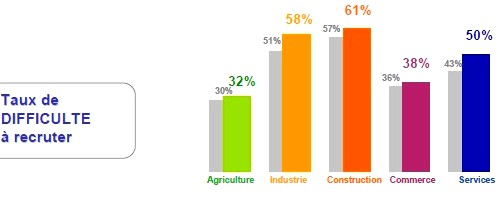
\includegraphics[trim=7cm 0cm 0cm 0cm, clip=true, width=0.5\textwidth]{../resources/illustrations/diff_recrut}
		};
		\node[anchor=north west,inner sep=0pt,] at ($(current page.north west)+(0.7cm,-8cm)$) {
			{\tiny \it \color{black!30} Difficultés à recruter en 2012 en Midi-Pyrénées}
		};
		\node[anchor=north west,inner sep=0pt] at ($(current page.north west)+(6.5cm,-3cm)$) {
			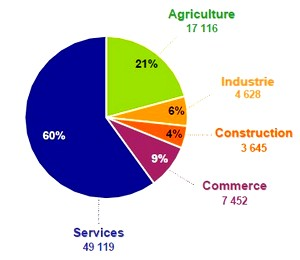
\includegraphics[width=0.5\textwidth]{../resources/illustrations/embauches}
		};
		\node[anchor=north west,inner sep=0pt,] at ($(current page.north west)+(6.5cm,-8cm)$) {
			{\tiny \it \color{black!30} Intentions d'embauche en 2012 en Midi-Pyrénées}
		};
	\end{tikzpicture}
	\footlineextra{\cite{recrutement_midi_pyr}}
\end{frame}


\subsection{Communication}

\begin{frame}{Embauches et internet}
	\begin{tikzpicture}[remember picture,overlay]
		\node[anchor=north west,inner sep=0pt] at ($(current page.north west)+(0.2cm,-1.7cm)$) {
			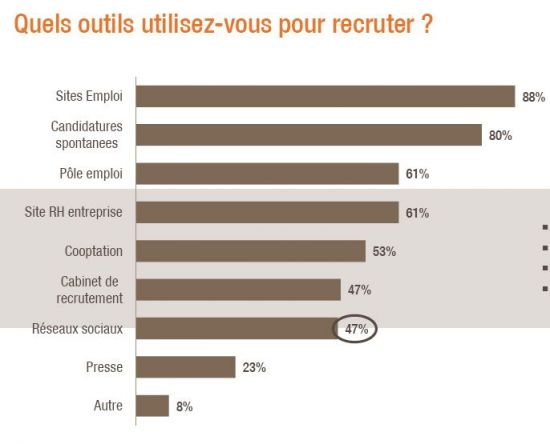
\includegraphics[trim=0cm 0cm 0cm 0cm, clip=true, width=.6\textwidth]{../resources/illustrations/recrutement-enquete}
		};
		\node[anchor=north west,inner sep=0pt] at ($(current page.north west)+(6cm,-3.5cm)$) {
			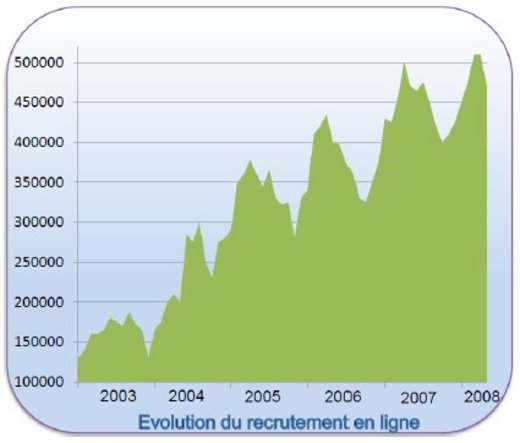
\includegraphics[trim=0cm 0cm 0cm 0cm, clip=true, width=.6\textwidth]{../resources/illustrations/online_recrut}
		};
	\end{tikzpicture}
	
	\footlineextra{\cite{recrutement_internet}\cite{recrut_social_network}\cite{social_recrut}}
\end{frame}

\begin{frame}{Réseaux sociaux et chantage}
	\includegraphicsabsolute{../resources/illustrations/Amanda_Todd}{.6\textwidth}{0.2cm}{1.7cm}
	\includegraphicsabsolute{../resources/illustrations/facebook_blackmail}{.6\textwidth}{6cm}{4.7cm}
	\footlineextra{\cite{chantage_facebook}\cite{harcel_facebook}}
\end{frame}

\subsection{Décrochages et échecs scolaires}

\begin{frame}{Formation inadaptée}
	\begin{tikzpicture}[remember picture,overlay]
		\node[anchor=north west,inner sep=0pt] at ($(current page.north west)+(0.5cm,-1.5cm)$) {
			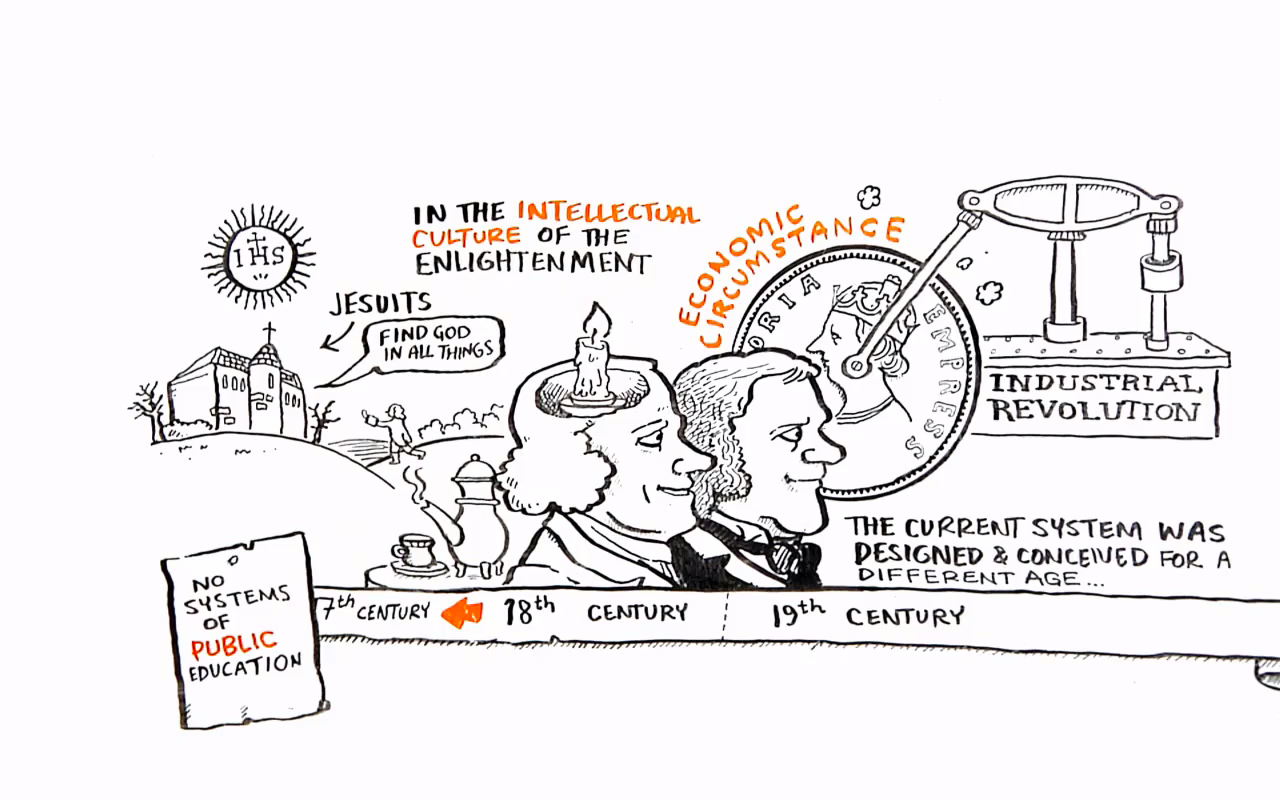
\includegraphics[trim=2cm 1.5cm 0cm 1.5cm, clip=true, width=\linewidth]{../resources/illustrations/public_education}
		};
	\end{tikzpicture}
	\footlineextra{\cite{robinson2010paradigms}}
\end{frame}

\begin{frame}{Troubles de l'attention}
	\begin{tikzpicture}[remember picture,overlay]
		\node[anchor=north west,inner sep=0pt] at ($(current page.north west)+(1.5cm,-1.5cm)$) {
			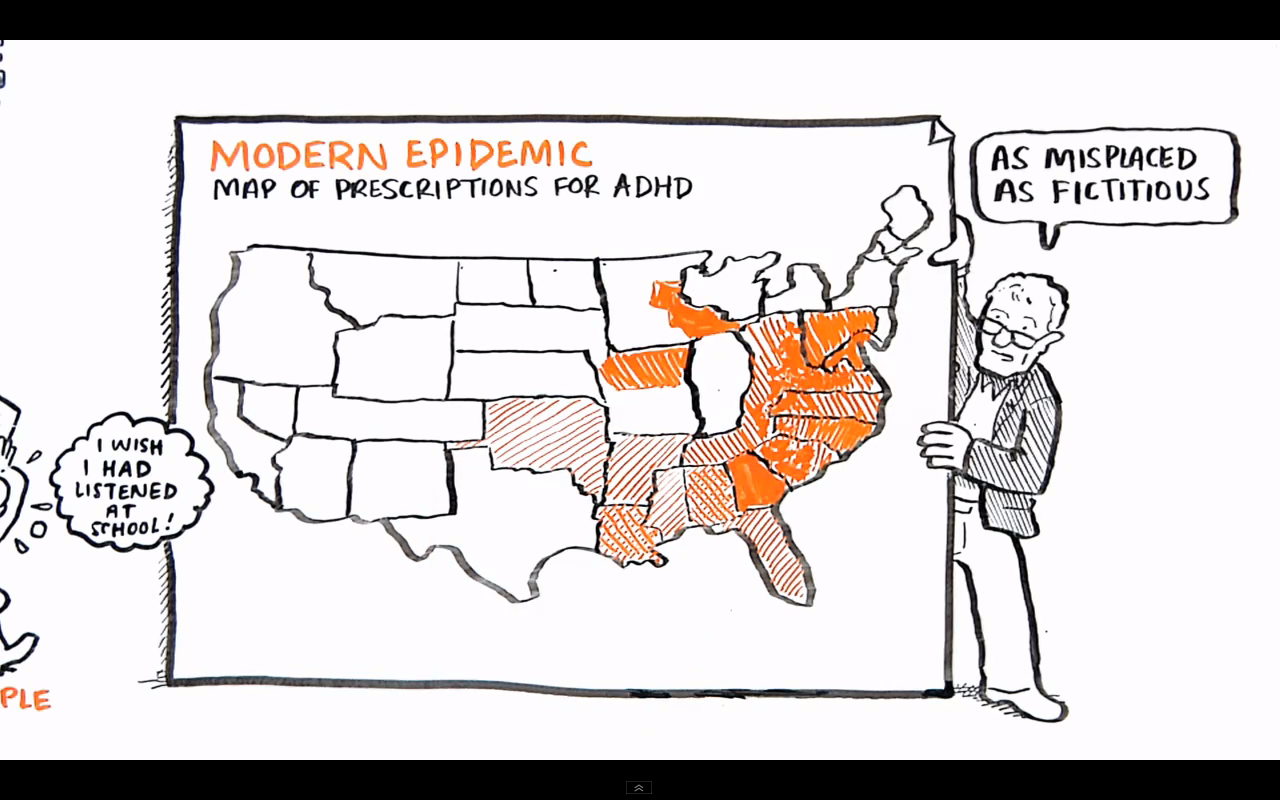
\includegraphics[trim=1.9cm 1.5cm 0cm 1.5cm, clip=true, width=\linewidth]{../resources/illustrations/ADHD}
		};
	\end{tikzpicture}
	\footlineextra{\cite{robinson2010paradigms}}
\end{frame}


